\documentclass[8pt,xcolor=svgnames]{beamer}
\usepackage{paquetes}
\usepackage{modo}

\usepackage{minted}
\usemintedstyle{tango}
\definecolor{bg}{rgb}{0.95,0.95,0.95}
\newminted{cpp}{bgcolor=bg}

\setlength{\parskip}{0.4cm}

\begin{document}

% Transparencia de Inicio -> Título
\begin{frame}
  \titlepage
\end{frame}


\normalsize

% % Transparencia de índice
% \begin{frame}
%   \frametitle{Índice} 
%   % \transboxin
%   \tableofcontents
% \end{frame}


\section{Introducción}

\subsection{Qué es C++11, qué es Boost}

\begin{frame}

  \begin{block}{¿Qué es C++?}
    Bitch, please.   
  \end{block}

  \pause

  \begin{block}{¿Qué es C++11?}
    \begin{itemize}
    \item \textit{Nuevo} estándar de C++.
    \item Nuevos elementos sintácticos.
    \item Nuevas bibliotecas.
    \item Objetivo: \textit{``simplificar el uso y la enseñanza de C++''}.
    \end{itemize}
  \end{block}

  \pause

  \begin{block}{¿Qué es Boost?}
    \begin{itemize}
    \item Bibliotecas (80+) de código abierto y revisión por pares para C++.
    \item Escritas por los mejores programadores C++. Revisión por pares.
    \item 12 de estas librerías se han integrado en C++: Array,
      Bind, Function, Hash, mem\_fn, Random, Ref, Regex, Smart Pointers, Tuple,
      Type Traits y Unordered.
    \item Muchas son \textit{header only}.
    \end{itemize}
  \end{block}
\end{frame}

\subsection{¿Cómo va la charla?}

\begin{frame}{¿Cómo va a ir la charla?}
  \centering

  Repaso de lo nuevo de C++11, comentando qué partes vienen de Boost.

\pause

\begin{block}{Compilar}
  Usar la opción \texttt{-std=c++11} en GCC o Clang.
\end{block}
  
\end{frame}

\section{¿Qué hay de nuevo, viejo?}

\begin{frame}
  \Huge 
  \centering

  ¿Qué hay de nuevo, viejo?

\end{frame}

\subsection{Deducción de tipos}

\begin{frame}[fragile]{Deducción de tipos}

Por ejemplo, tenemos un mapa:
\begin{cppcode}
std::map<string, std::vector<int> > m;
\end{cppcode}

\pause

Pillemos un iterador...
\begin{cppcode}
std::map<string, std::vector<int> >::reverse_iterator i = m.rbegin();    
\end{cppcode}

\pause
\textbf{¡NOR!}
\pause

\begin{cppcode}
auto i = m.rbegin();  
\end{cppcode}

\end{frame}

\subsection{Inicialización uniforme}

\begin{frame}[fragile]{Inicialización uniforme}
Antiguamente podías hacer esto para tipos POD:

\begin{cppcode}
int a[] = { 1, 2, 3, 4 };  
\end{cppcode}

\pause

Ahora es posible hacerlo con cualquier tipo de datos:

\begin{cppcode}
vector<string> v = { "Hola", "Hello" };  
\end{cppcode}

\pause 

Para implementarlo en nuestras clases, definir un nuevo constructor:

\begin{cppcode}
MiClase(const std::initializer_list<int> & x) {
    // Inicializar la clase con los valores de x
}  
\end{cppcode}
\end{frame}

\subsection{Bucles basados en rangos}
\begin{frame}[fragile]{Bucles basados en rangos}

¿Iterar por un vector?

  \begin{cppcode}
vector<int> v { 3, 4 };

for(vector<int>::iterator i = v.begin(); i != v.end(); ++i) {
    cout << *i << endl;
}
  \end{cppcode}

\pause

\textbf{Nope}. Chuck testa.

\begin{cppcode}
for ( auto i : v ) {
    cout << i << endl;
}
\end{cppcode}
\end{frame}

\begin{frame}[fragile]{Bucles basados en rangos - Modificación de elementos}
 ¿Y si quiero modificar los elementos del contenedor? NO PROB.  

 \begin{cppcode}
for ( auto & i : v ){ // Ojo a la referencia
    i = 2 * i;
}   
 \end{cppcode}
\end{frame}

\subsection{Constante para puntero nulo}

\begin{frame}[fragile]{Constante para puntero nulo}

  En C++, \texttt{NULL} equivale a 0, lo que da lugar a ambigüedades, por
  ejemplo:

  \begin{cppcode}
void foo(char *);
void foo(int);

foo(NULL);    
  \end{cppcode}

  En ese caso se llamaría a \texttt{foo(int)} en vez de
  \texttt{foo(char*)}. 

  Para evitar eso, a partir de ahora usar \texttt{nullptr}:

  \begin{cppcode}
foo(nullptr);    
  \end{cppcode}
  
\end{frame}

\subsection{Tablas hash}

\begin{frame}[fragile]{Tablas hash}

  \centering

  Por fin, contenedores basados en tablas hash, formalmente \textit{contenedores
    asociativos desordenados}. Estos son:

  \textbf{\texttt{unordered\_set, unordered\_multiset, \\ unordered\_map, unordered\_multimap}}.

  Portados de \texttt{boost::unordered}.

  Tiempo medio en $O(1)$
  
\end{frame}

\subsection{Expresiones regulares}

\begin{frame}[fragile]{Expresiones regulares}

\centering

¡Expresiones regulares! Futurista total, ni que estuviéramos en el siglo XXI.

Portadas de \texttt{boost::regex}. 

El soporte de los compiladores es \textit{regulá}, mejor usar Boost.
 
\end{frame}

% \begin{frame}[fragile]{Expresiones regulares, tipos de datos}
 
%   \begin{block}{Secuencia objetivo}
%     Normalmente un \texttt{std::string}.
%   \end{block}

%   \begin{block}{Patrón}
%     Definido con \texttt{std::regex} (ó \texttt{boost::regex}).
%   \end{block}
  
%   \begin{block}{Resultados}
%     Guardan el resultado del procedimiento. 
%     \begin{itemize}
%     \item \texttt{std::cmatch} para \texttt{char *}
%     \item \texttt{std::smatch} para \texttt{std::string}
%     \end{itemize}    
%   \end{block}  
% \end{frame}

% \begin{frame}[fragile]{Expresiones regulares, funciones}

%   \begin{itemize}
%   \item \texttt{regex\_match} y \texttt{regex\_search}: coincidencia total o parcial.
%   \end{itemize}
  
% \end{frame}

\begin{frame}[fragile]{Expresiones regulares, ejemplo}
  \begin{cppcode}
boost::regex exp(".*\\.jpe?g");

std::string ficheros[] = 
  { "doc.pdf", "img1.jpg", "gurl.jpeg", "file.txt" };
    
for (auto & f : ficheros) {
    if (boost::regex_match(f, exp)) {
        cout << f << " es una imagen." << endl;
    } else {
        cout << f << " no es una imagen." << endl;
    }
}    
  \end{cppcode}
\end{frame}

\subsection{Smart pointers}

\begin{frame}

\centering

\begin{figure}[c!]
  \centering
  
\includegraphics{img_memory_leaks.jpg}

  \Huge \textbf{Nunca más}
\end{figure}  
\end{frame}

\begin{frame}[fragile]{Smart pointers}

  No tendrás que hacer \texttt{new} y \texttt{delete} nunca más gracias a los
  \textbf{\texttt{smart pointers}}. \\Hay varios tipos:

  \begin{itemize}
  \item \textbf{\texttt{unique\_ptr}}: puntero único a un recurso, nadie más puede apuntar
    a él. Cuando se destruye el puntero, el recurso se libera.
  \item \textbf{\texttt{shared\_ptr}}: puntero a un recurso que puede ser
    compartido por más \texttt{shared\_ptr}. Cuando ningún \texttt{shared\_ptr}
    apunta al recurso, éste se libera.
  \item \textbf{\texttt{weak\_ptr}}: puntero débil, es como un
    \texttt{shared\_ptr} pero no se tiene en cuenta al contar referencias.
  \end{itemize}
  
Basados en \texttt{boost::smart\_pointers}.
\end{frame}

\begin{frame}[fragile]{Smart pointers, ejemplo}

  \begin{cppcode}
struct ClaseGordisima { 
    ~ClaseGordisima() { cout << "Me destruyen!" << endl; }
};

void foo (ClaseGordisima & p) { /* ... */ }

int main()
{
    unique_ptr<ClaseGordisima> puntero { new ClaseGordisima };
    foo(*puntero);
} 
// Al salir del scope se libera el recurso   
  \end{cppcode}
  
\end{frame}

\begin{frame}[fragile]{Smart pointers, ejemplo con shared\_ptr}

  \begin{cppcode}
struct Poseido { 
    ~Poseido() { cout << "Bye :(" << endl; }
};

struct Poseedor {
    shared_ptr<Poseido> puntero;
};

int main() 
{
    deque<Poseedor> p;
    p.push_back(Poseedor());
    p.push_back(Poseedor());

    p[0].puntero.reset(new Poseido);
    p[1].puntero = p[0].puntero;      // 1

    p.pop_front();    // 2
    p.pop_front();    // 3
}    
  \end{cppcode}
  
\end{frame}

\subsection{Funciones lambda}

\begin{frame}[fragile]{Funciones lambda}
\centering

Nueva sintaxis para definir funciones lambda:

\begin{cppcode}
auto func = [] () { cout << "Hello world"; };
func();

auto func2 = [] (int a) { return 2 * a; };
func2(4);

int something = 5;
auto func3 = [something] (int a) { return something * a; }
func3(4);

\end{cppcode}

\end{frame}

\begin{frame}[fragile]{Ejemplo lambda}

\begin{cppcode}
struct Person {
    string name;
    enum { MALE, FEMALE } gender;
};

int main(int argc, char *argv[])
{
    Person p1 { "Jose", Person::MALE };
    Person p2 { "Leti", Person::FEMALE };

    vector<Person> people { p1, p2 };

    size_t num_females = count_if(people.begin(), people.end(), 
         [] (Person & p) { return p.gender == Person::FEMALE; });

    cout << "Hay " << num_females << " chicas." << endl;
}  
\end{cppcode}
  
\end{frame}


\subsection{Bind y Function}

\begin{frame}{Facilidades para trabajar con functors}
  C++11 renueva las herramientas para trabajar con funciones objeto, la mayoría
  copiadas de \texttt{boost} (MOAR FUNCTIONAL PLS KTHXBYE):

  \begin{itemize}
  \item \texttt{std::function}, wrapper genérico para cosas
    \textit{``llamables''} (funciones, clases con \texttt{operator()}
  \item \texttt{std::bind}, crea wrappers para \textit{callables} con algunos
    argumentos \textit{bindeados} (toma ya). Mejor ver el ejemplo.
  \end{itemize}

\end{frame}

\begin{frame}[fragile]{Aplicaciones parciales}

Por ejemplo, aplicaciones parciales:

\begin{cppcode}
#include <functional>
using namespace std::placeholders;

float aplicarIVA (float base, float IVA) {
    return base + IVA * base;
}

int main(int argc, char *argv[])
{
    auto aplicarIVA21 = std::bind(aplicarIVA, _1, 0.21);
    cout << "5 euros + IVA = " << aplicarIVA21(5) << "euros \n";
}  
\end{cppcode}
  
\end{frame}

\begin{frame}
  \begin{figure}[c!]
    \centering
    
\includegraphics[width=\textwidth]{img_doge_functional.jpg}
  \end{figure}
\end{frame}

\subsection{Concurrencia}

\begin{frame}[fragile]{Soporte para threading}
  Ahora C++11 tiene soporte para threading de manera uniforme entre plataformas:

  \begin{cppcode}
#include <thread>

void task1(string msg) {
    cout << "task1 says: " << msg;
}

int main(){
    thread t1(task1, "Hello");

    t1.join();
}    
  \end{cppcode}

También viene con sus mutex, sus locks, etc. Tó la pesca.
  
\end{frame}

\begin{frame}
  \begin{figure}[c!]
    \centering
    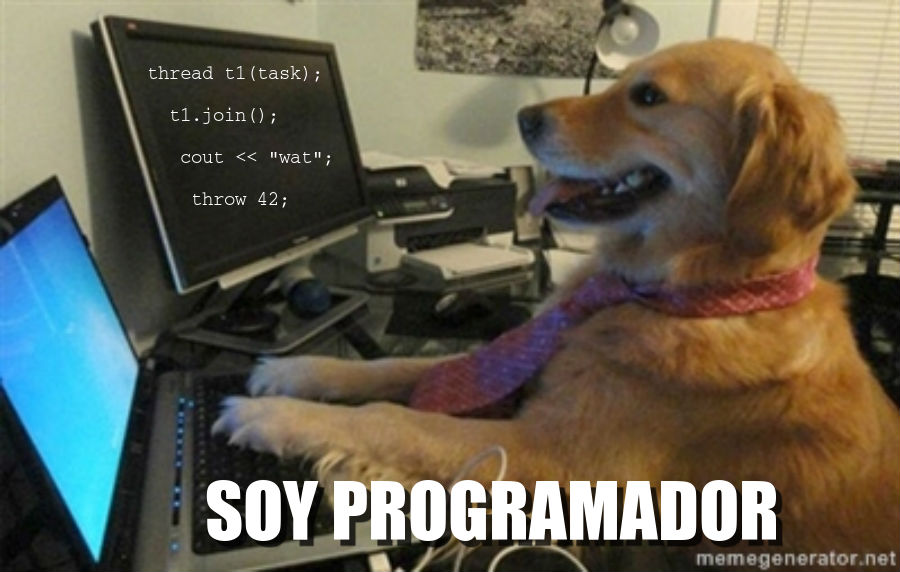
\includegraphics[width=\textwidth]{img_dog_throw.jpg}
  \end{figure}
\end{frame}

\begin{frame}[fragile]{Promesas de futuro}

  Se añaden nuevas construcciones de alto nivel para tareas asíncronas, para no
  mancharnos las manos con hilos. Por ejemplo, \texttt{std::async}:

  \begin{cppcode}
 int fun(int b) { /* Calculo cosas que tardan bastante */ }

 int main () {
     auto fun_futuro = std::async(fun, 20);

     // Hago otras cosas

     int resultado = fun_futuro.get();
 }

   \end{cppcode}

\end{frame}

%%%%%%%%%%%%%%%%%%%%%%%%%%%%%%%%%%%%%%%%%%%%%%%%%%%%

\section{Conclusiones}

\begin{frame}{Otras cosas de C++11}
  \begin{itemize}
  \item \texttt{std::ref} (de boost)
  \item \texttt{std::hash} (de boost)
  \item \texttt{std::tuple} (de boost)
  \item Expresiones constantes: \texttt{constexpr}
  \item Referencias a rvalues (\texttt{T\&\&}) y semántica de movimiento.
  \item Delegación de constructores.
  \item Indicación explícita de sobrecargas y métodos finales.
  \item Indicación explícita de métodos borrados y predeterminados.
  \item Plantillas \textit{variadic}.
  \item Nuevos literales de cadena con soporte para UTF (8, 16, 32).
  \item Literales defindos por el usuario, para hacer tus propias \textit{``unidades''}.
  \item Asertos en tiempo de compilación.
  \item Motor de distribuciones aleatorias.
  \end{itemize}  
\end{frame}

\begin{frame}{Otras cosas de Boost}
  \begin{itemize}
  \item \texttt{boost::lexical\_cast}
  \item \texttt{boost::any}
  \item \texttt{boost::format}
  \item \texttt{boost::filesystem}
  \item \texttt{boost::multiindex}
  \item \texttt{boost::signals}
  \item \texttt{boost::spirit} (EBNF)
  \end{itemize}  
\end{frame}

\begin{frame}{Más sobre Boost}

\centering

\Huge

Más sobre boost en:

\large

\texttt{https://github.com/JoseTomasTocino/boost-workshop}
  
\end{frame}

\begin{frame}{}
  \begin{figure}[c!]
    \centering
    
\includegraphics[width=0.5\textwidth]{img_cat_bye.jpg}
  \end{figure}
\end{frame}

% % \subsubsection{Boost.Bind}

% \begin{frame}[fragile]{Boost.Bind}
%   \begin{block}{}
%     \textit{bind: } envolver, vendar, atar, amarrar, ligar.
%   \end{block}
%   \begin{block}{boost::bind}
%     \texttt{boost::bind} es una generalización de \texttt{std::bind1st} y
%     \texttt{std::bind2nd}. Nos permite \textit{bindear} una serie de
%     argumentos a cualquier cosa que \textit{tenga pinta de función}:
%     punteros a función, objetos función, y punteros a función-miembro.
%   \end{block}

%   \pause
%   \begin{center}
%     {\huge What?}
%   \end{center}

%   \pause

%   \begin{block}{}
%     La veremos en la segunda parte del taller.
%   \end{block}
% \end{frame}

% % \subsubsection{Boost.Function}

% \begin{frame}{Boost.Function}
%   \begin{block}{boost::function}
%     \texttt{boost::function} nos proporciona \textit{alojamiento} de funciones,
%     funciones objeto y funciones miembro para su posterior
%     ejecución. Se suele utilizar en conjunto con Boost::bind.
%   \end{block}

%   \pause

%   \begin{block}{}
%     La veremos en la segunda parte del taller.
%   \end{block}  
% \end{frame}

% % \subsubsection{Boost.Hash}

% \begin{frame}{Boost.Hash}
%   \begin{block}{}
%     \texttt{boost/functional/hash.hpp}
%   \end{block}
%   \begin{block}{boost::hash}
%     \texttt{boost::hash} nos permite generar hashes para enteros, flotantes,
%     punteros y cadenas de forma nativa, y además provee soporte para
%     la generación de hashes para tipos de datos definidos por el
%     usuario y contenedores.
%   \end{block}
%   \pause
%   \begin{block}{}
%     Veamos el ejemplo en \texttt{ejemplos\_tr1/boost\_hash}
%   \end{block}
% \end{frame}

% % \subsubsection{Boost.Mem\_fn}

% \begin{frame}{Boost.Mem\_fn} 
%   \begin{block}{}
%     \texttt{boost/mem\_fn.hpp}
%   \end{block}
%   \begin{block}{boost::mem\_fn}
%     \texttt{boost::mem\_fn} se podría definir como un caso concreto de
%     \texttt{boost::bind}. Sirve para generar objetos función que
%     apuntan a funciones miembro. De ahí el nombre: mem\_fn = member
%     function.
%   \end{block}
%   \pause
%   \begin{block}{Acerca del solapamiento con bind}
%     \url{http://stackoverflow.com/questions/3088058/whats-the-point-of-using-boostmem-fn-if-we-have-boostbind}
%   \end{block}
%   \pause
%   \begin{block}{}
%     Veamos el ejemplo en \texttt{ejemplos\_tr1/boost\_mem\_fn}
%   \end{block}  
% \end{frame}

% % \subsubsection{Boost.Random}

% \begin{frame}{Boost.Random}
%   \begin{block}{}
%     \texttt{boost/random/*}
%   \end{block}
%   \begin{block}{boost::random}
%     \texttt{boost::random} sirve, como su nombre indica, para trabajar
%     con números aleatorios. Proporciona una serie de generadores
%     aleatorios, de diferente eficiencia, y un conjunto de
%     distribuciones a las que podemos mapear la salida de los
%     generadores para facilitar las cosas, en lugar de andar nosotros
%     haciendo el módulo y tal.
%   \end{block}  
%   \pause
%   \begin{block}{}
%     Veamos el ejemplo en \texttt{ejemplos\_tr1/boost\_random}
%   \end{block}  
% \end{frame}

% % \subsubsection{Boost.Ref}

% \begin{frame}{Boost.Ref}
%   \begin{block}{}
%     \texttt{boost/functional/ref.hpp}
%   \end{block}
%   \begin{block}{boost::ref}
%     \texttt{boost::ref} sirve para pasar referencias a funciones que
%     normalmente tomarían sus argumentos por valor. Así evitamos la
%     duplicación, que en algunos casos no es posible.
%   \end{block}
%   \begin{alertblock}{Disclaimer}
%     No he podido dedicarle tiempo, así que no tengo mucha idea del
%     tema.
%   \end{alertblock}
% \end{frame}

% % \subsubsection{Boost.Regex}

% \begin{frame}{Boost.Regex}
%   \begin{block}{boost::regex}
%     \texttt{boost::regex} es una biblioteca de expresiones regulares
%     que veremos en la segunda parte del taller.
%   \end{block}
% \end{frame}

% % \subsubsection{Boost Smart Pointers}

% \begin{frame}{Boost Smart Pointers}
%   \begin{block}{Boost Smart Pointers}
%     Los \texttt{smart pointers} de boost son una serie de punteros
%     inteligentes que se ocupan automáticamente de la gestión de la
%     vida de los objetos, ahorrándonos tener que liberar la memoria al
%     terminar de usarlos
%   \end{block}
%   \begin{block}{}
%     La veremos en la segunda parte del taller.
%   \end{block}  
% \end{frame}

% % \subsubsection{Boost.Tuple}

% \begin{frame}{Boost.Tuple}
%   \begin{block}{}
%     \texttt{boost/tuple/*}
%   \end{block}
%   \begin{block}{boost::tuple}
%     \texttt{boost::tuple} es una especie de versión generalizada de
%     \texttt{std::pair}, en la que se puede almacenar un número
%     arbitrario de valores de distinto tipo. Es especialmente útil
%     cuando necesitamos que una función devuelva varios valores.
%   \end{block}
%   \pause
%   \begin{block}{}
%     Veamos el ejemplo en \texttt{ejemplos\_tr1/boost\_tuple}
%   \end{block}  
% \end{frame}

% % \subsubsection{Boost.TypeTraits}

% \begin{frame}{Boost.TypeTraits}
%   \begin{block}{}
%     \texttt{boost/type\_traits.hpp}
%   \end{block}
%   \begin{block}{Background}
%     Una \texttt{trait class} es una clase paramétrica que ofrece información
%     sobre un tipo de datos en tiempo de compilación. (trait = rasgo)
%   \end{block}
%   \pause
%   \begin{block}{boost.typetraits}
%     Se trata de una colección de clases trait que nos ayudarán a la
%     hora de caracterizar un tipo de datos cuando trabajemos con
%     programación genérica, pudiendo adaptar nuestros algoritmos según
%     las propiedades del tipo de datos pero manteniendo la genericidad.
%   \end{block}
%   \pause
%   \begin{block}{}
%     Veamos el ejemplo en \texttt{ejemplos\_tr1/boost\_typetraits}
%   \end{block}  
% \end{frame}

% % \subsubsection{Boost.Unordered}

% \begin{frame}{Boost.Unordered}
%   \begin{block}{}
%     \texttt{boost.unordered} proporciona alternativas no ordenadas a
%     \texttt{set}, \texttt{map}, \texttt{multiset} y \texttt{multimap},
%     basándose en \texttt{boost::hash} para crear una tabla hash,
%     mejorando el rendimiento en el acceso a los elementos.
%   \end{block}
%   \pause
%   \begin{block}{boost/unordered\_set.hpp}
%     Proporciona los tipos \texttt{boost::unordered\_set} y
%     \texttt{unordered\_multiset}.
%   \end{block}
%   \pause
%   \begin{block}{boost/unordered\_map.hpp}
%     Proporciona los tipos \texttt{boost::unordered\_map} y
%     \texttt{unordered\_multimap}.
%   \end{block}
%   \pause
%   \begin{block}{}
%     Veamos el ejemplo en \texttt{ejemplos\_tr1/boost\_unordered}
%   \end{block}  
% \end{frame}

% \section{Segunda parte: bibliotecas útiles de Boost}
% \subsection{boost::format}

% \begin{frame}{boost::format}
%   \begin{block}{}
%     \texttt{boost/format.hpp}
%   \end{block}
%   \begin{block}{boost::format}
%     Nos permite formatear cadenas utilizando la sintaxis típica de printf.

%     \begin{itemize}
%     \item Utiliza un flujo interno en el que vuelca los argumentos
%     \item Utiliza el operador \% para pasar los valores.
%     \end{itemize}
%   \end{block}

%   \begin{block}{Sintaxis básica}
%     \texttt{boost::format( cadena-formato ) \% arg1 \% arg2 \% ... \% argN}    
%   \end{block}

%   \begin{block}{También como objeto}
%     \texttt{boost::format miFormato(" ... ");} \\
%     \texttt{miFormato \% valor1 \% valor2; }
%   \end{block}
% \end{frame}

% \begin{frame}{boost::format}
%   \begin{block}{Sintaxis de la cadena de formato}
%     Compuesta de bloques que definen el formato de cada argumento:
%     \begin{itemize}
%     \item \texttt{\%spec} Forma clásica de printf.
%     \item \texttt{\%|spec|}  Como la anterior pero no es necesario indicar el tipo de datos.
%     \item \texttt{\%N\%} Forma simple, sólo se indica la posición del argumento.
%     \end{itemize}    
%   \end{block}

%   \begin{block}{Sintaxis de \texttt{spec}}
%     \texttt{[ N\$ ][ flags ][ ancho ][ .precisión ][caracter-de-tipo]}    
%     \begin{itemize}
%     \item \texttt{[ N\$ ]} Referencia al argumento N-ésimo.
%     \item \texttt{[ flags ]} Posibles banderas de formato:
%       {\scriptsize
%         \begin{itemize}
%         \item \texttt{'-'}  alineación a la izquierda.
%         \item \texttt{'='}  alineación centrada.
%         \item \texttt{'\_'}  alineación interna.
%         \item \texttt{'+'}  mostrar signo incluso para números positivos.
%         \item \texttt{'0'}  rellenar con ceros.
%         \end{itemize}
%       }
%     \item \texttt{[ ancho ]} ancho mínimo. Relleno con espacios.
%     \end{itemize}
%   \end{block}
% \end{frame}

% \begin{frame}[fragile]{boost::format}
%   \begin{block}{Tabulación absoluta}
%     \begin{itemize}
%     \item \texttt{\%|nt|} siendo \texttt{n} un entero, indica que se
%       utilizarán caracteres de relleno si es necesario para que la cadena
%       esté a \texttt{n} caracteres del inicio.
%     \item \texttt{\%|nTX|} igual que en el caso anterior, pero X indicará
%       el caracter de relleno.
%     \end{itemize} 
%     Se escribe antes de cada cadena \texttt{spec}.
%   \end{block}
% \end{frame}

% \begin{frame}[fragile]{boost::format Ejemplos}
%   \begin{block}{}
%     {\scriptsize
% \begin{verbatim}
% // argumentos por posición
% // format("%|2$| %1$i \n") % "11" % "hola";

% hola 11

% // alineación centrada, ancho 15
% // format("|%|=15||%|=15||%|=15||\n") % "Oficina" % "Software" % "Libre";

% |    Oficina    |    Software   |     Libre     |

% // Tabulación absoluta
% // format("%2% %|10t|%|1$| \n") % "Godofredo" % "A1";    
% // format("%2% %|10t|%|1$| \n") % "Godofredo" % "A12345";

% A1        Godofredo 
% A12345    Godofredo

% // Notación de números
% // format("%|30.5| \n") % 12312344.42345823904;
% // format("%|+30.5| \n") % 12312344.42345823904;  
% // format("%|+30.5e| \n") % 12312344.42345823904; 
% // format("%|+30.5f| \n") % 123123.42345823904;   

%                     1.2312e+07 
%                    +1.2312e+07 
%                   +1.23123e+07 
%                  +123123.42346 
% \end{verbatim}
      
%     }
%   \end{block}
% \end{frame}

% \subsection{boost::regex}
% \begin{frame}{boost::regex}
%   \begin{block}{}
%     \texttt{boost/regex.hpp}
%   \end{block}
%   \begin{block}{Expresiones regulares}
%     Las expresiones regulares son unas expresiones que sirven para
%     desribir conjuntos de cadenas. Utilizan una sintaxis bastante
%     normalizada, y su utilidad se centra en buscar y manipular textos.
%   \end{block}
%   \pause
%   \begin{block}{boost::regex}
%     Ofrece soporte para búsquedas y reemplazos en textos usando
%     expresiones regulares de manera muy sencilla e intuitiva.
%   \end{block}
%   \pause
%   \begin{alertblock}{Enlazado}
%     Es una de las pocas bibliotecas de Boost que necesita de
%     enlazado: \texttt{-lboost\_regex}
%   \end{alertblock}
% \end{frame}

% \begin{frame}[fragile]{Tipos de datos}
%   \begin{block}{boost::regex}
%     \texttt{boost::regex} se usa para definir la expresión
%     regular. Viene en dos versiones: \texttt{regex} y \texttt{wregex}.
% \begin{verbatim}
%        boost::regex patron("\\w+(\\s+\\w+){2,}\\s*");
% \end{verbatim}
%   \end{block}

%   \pause

%   \begin{block}{boost::match\_results}
%     \texttt{match\_results} es una clase paramétrica que guarda
%     información sobre las ocurrencias encontradas al realizar una
%     operación con una expresión regular.
    
%     \begin{itemize}
%     \item \texttt{cmatch} para char *
%     \item \texttt{wcmatch} para wchar *
%     \item \texttt{smatch} para string
%     \item \texttt{wsmatch} para wstring
%     \end{itemize}
%   \end{block}
% \end{frame}

% \begin{frame}[fragile]{Funciones libres}
%   \begin{block}{Coincidencia total}
%     \texttt{boost::regex\_match} nos sirve para ver si una cadena
%     concuerda \textbf{en su totalidad} con una expresión regular.
% \begin{verbatim}
% bool boost::regex_match(cadena, resultado, patrón);
% \end{verbatim}
%   \end{block}

%   \pause
%   \begin{block}{Coincidencia parcial}
%     \texttt{boost::regex\_search} se usar para buscar alguna
%     coincidencia de la expresión regular dentro de una cadena.
% \begin{verbatim}
% bool boost::regex_search(cadena, resultado, patrón);
% \end{verbatim}
%   \end{block}
  
%   \pause
%   \begin{block}{Reemplazo}
%     \texttt{boost::regex\_replace} reemplaza ocurrencias de la
%     expresión regular en la cadena con otra en el formato que
%     indiquemos.
    
% \begin{verbatim}
% string boost::regex_replace(cadena, patron, reemplazo);      
% \end{verbatim}

%   \end{block}

% \end{frame}

% \begin{frame}{Iteradores}
%   \begin{block}{boost::regex\_iterator}
%     \texttt{boost::regex\_iterator} nos permitará iterar sobre las
%     ocurrencias de una expresión regular sobre una cadena.
%   \end{block}
  
%   \pause

%   \begin{block}{boost::regex\_token\_iterator}
%     \texttt{boost::regex\_token\_iterator} nos puede servir para
%     tokenizar una cadena, usando un patrón como divisor.
%   \end{block}

%   \pause
%   \begin{block}{}
%     Ambos iteradores vienen en cuatro sabores, según el tipo de
%     caracter que se use. En nuestros ejemplos usaremos
%     \texttt{std::string}, así que habría que anteponer una \textit{s}
%     a los nombres de los tipos
%   \end{block}
% \end{frame}

% \subsection{boost::program\_options}

% \begin{frame}{boost::program\_options}
%   \begin{block}{}
%     \texttt{boost/program\_options.hpp}
%   \end{block}
%   \begin{block}{boost::program\_options}
%     \texttt{boost::program\_options} nos permite parsear, de manera
%     sencilla, efectiva y segura, los argumentos que le pasemos a los
%     programas al ejecutarlos en la línea de comandos, así como parsear
%     ficheros de configuración y variables de entorno.
%   \end{block}
%   \pause
%   \begin{alertblock}{Enlazado}
%     Es otra de las pocas bibliotecas de Boost que necesita de
%     enlazado: \texttt{-lboost\_program\_options}
%   \end{alertblock}
% \end{frame}

% \begin{frame}{Modularización}
%   \begin{block}{Modularización}
%     El proceso de parseo tiene tres partes:
%     \begin{itemize}
%     \item Descripción sintáctica y semántica de las opciones y argumentos.
%     \item Parseo de la entrada, ya sea de la línea de comandos o de otro origen.
%     \item Almacenamiento en un mapa de variables o usando referencias.
%     \end{itemize}
%   \end{block}  
% \end{frame}

% \begin{frame}{Definición de opciones}
%   \begin{block}{}
%     \texttt{namespace po = boost::program\_options;}
%   \end{block}
%   \begin{block}{Opciones}
%     Los objetos \texttt{po::options\_description} guardan la
%     descripción de todas las opciones. Éstas suelen tener tres partes:
%     \begin{itemize}
%     \item \textbf{Sintaxis:} Nombre corto y largo.
%     \item \textbf{Semántica:} ¿Recibe valores?
%     \item \textbf{Descripción:} Información sobre la opción.
%     \end{itemize}
%   \end{block}
%   \pause
%   \begin{block}{Opciones posicionales}
%     Hay veces en las que incluímos argumentos que no pertenecen a
%     ninguna opción, sino que \textit{van por libre}. Los veremos en el
%     segundo ejemplo.
%   \end{block}
% \end{frame}

% \begin{frame}{Parseo y almacenamiento}
%   \begin{block}{Almacenamiento}
%     Se utilizará un tipo \texttt{po::variables\_map} para guardar las
%     opciones parseadas, que es un mapa multivalor (hace uso de
%     \texttt{boost::any}).
%   \end{block}
%   \pause
%   \begin{block}{Parseo}
%     Si no tenemos grandes pretensiones, podemos utilizar la función
%     libre \texttt{po::parse\_command\_line}, que nos devolverá las
%     opciones parseadas que podremos almacenar en el mapa de variables.

%     Para casos más elaborados podremos instanciar un parser, aplicarle
%     opciones y luego procesar la entrada (ejemplo 2).
%   \end{block}
%   \pause
%   \begin{block}{Acceso}
%     Las opciones, una vez parseadas, se guardan en el mapa de
%     variables, al que se puede acceder como un mapa cualquiera
%     (casteando los valores).
%   \end{block}
% \end{frame}

% \subsection{boost::foreach}

% \begin{frame}[fragile]{boost::foreach}
%   \begin{block}{}
%     \texttt{boost/foreach.hpp}
%   \end{block}
%   \begin{block}{boost::foreach}
%     Esta biblioteca hace proporciona exactamente lo que su nombre
%     indica: una forma fácil de iterar sobre un contenedor usando una
%     estructura \texttt{foreach}, presente en infinidad de lenguajes.

%     Proporciona una macro \texttt{BOOST\_FOREACH} que recibe dos
%     parámetros: el objeto en el que guardar el valor, y el contenedor
%     a recorrer:

% \begin{verbatim}
% std::string cadena("Hola mundo");
% BOOST_FOREACH(char c, cadena) {
%     std::cout << c;
% }
% \end{verbatim}
%   \end{block}
% \pause
%   \begin{block}{Tipos \textit{foreacheables}}
%     \begin{itemize}
%     \item Contenedores STL.
%     \item Arrays.
%     \item Cadenas terminadas en \texttt{NULL}.
%     \item Extendible a tipos del usuario.
%     \end{itemize}
%   \end{block}
% \end{frame}

% \begin{frame}[fragile]{}
%   \begin{block}{Recorrido inverso}
%     También existe \texttt{BOOST\_REVERSE\_FOREACH}, para iterar del
%     final al principio.
%   \end{block}
%   \pause
%   \begin{block}{Poniéndolo bonito}
%     Para evitar tener que usar la macro con mayúsculas, los \texttt{define} recomendados por \texttt{boost} son:
% \begin{verbatim}
% #define foreach         BOOST_FOREACH
% #define reverse_foreach BOOST_REVERSE_FOREACH
% \end{verbatim}
%   \end{block}
%   \pause
%   \begin{block}{Problemas conocidos}
%     \begin{itemize}
%     \item Los tipos de datos \textbf{con comas} suelen dar problemas,
%       ya que teóricamente la única coma que debe haber es la que
%       separa los dos argumentos del \texttt{foreach}. Para usar tipos
%       con comas (como \texttt{std::pair}), lo mejor es usar un typedef
%       antes.
%     \item \texttt{boost::foreach} está implementado usando
%       internamente \textbf{iteradores}, por lo que la adición o
%       eliminación de elementos al contenedor que estemos recorriendo
%       con \texttt{foreach} da lugar a la invalidación de los
%       iteradores previamente definidos, lo que suele conllevar un
%       comportamiento errático en tiempo de ejecución.
%     \end{itemize}
%   \end{block}
% \end{frame}

% \subsection{boost::lexical\_cast}

% \begin{frame}[fragile]{boost::lexical\_cast}
%   \begin{block}{}
%     \texttt{boost/lexical\_cast.hpp}
%   \end{block}
%   \begin{block}{Background}
%     ¿Cuántas veces hemos buscado en Google \textit{``string to int''}?
%     ¿Cuántas veces has mirado la sintaxis de un \texttt{stringstream}?
%     ¿Sabes qué significa la 'a' en \texttt{atoi}?

%     \medskip

%     Las conversiones léxicas son un tema peliagudo y recurrente,
%     \texttt{boost::lexical\_cast} ofrece una solución genérica que
%     funciona, fácil de usar y recordar, y con un impacto mínimo en
%     rendimiento y tamaño del ejecutable.
%   \end{block}
% \pause
%   \begin{block}{Sintaxis}
%     Básicamente, la sintaxis es la siguiente:

% \begin{verbatim}
% tipoDestino lexical_cast<tipoDestino>(tipoOrigen & valor);
% \end{verbatim}

%     Esto, señores, es \textit{magia potagia}. Bueno, realmente no:
%     Básicamente, de forma interna se vierte el valor a convertir en un
%     flujo, que se utiliza para rellenar el tipo destino.
%   \end{block}
% \end{frame}

% \begin{frame}{Ampliación y errores}
%   \begin{block}{}
%     Puede utilizarse con cualquier tipo de datos, siempre y cuando se cumpla lo siguiente:
%     \begin{itemize}
%     \item El \texttt{tipoOrigen} debe tener definido el \texttt{operador <<}
%       para flujos.
%     \item El \texttt{tipoDestino} debe tener definido el \texttt{operador >>}
%       para flujos.
%     \item El \texttt{tipoDestino} debe poderse construir por copia y tener
%       constructor por defecto.
%     \end{itemize}
%   \end{block}

%   \pause

%   \begin{block}{Excepciones}
%     Cuando no se puede hacer la conversión, se lanza una excepción del tipo \texttt{bad\_lexical\_cast : public std::bad\_cast}.
%   \end{block}

%   \pause

%   \begin{block}{Casts entre tipos numéricos}
%     Para convertir entre tipos numéricos, en especial tipos de
%     diferente ancho, es mejor usar \texttt{boost::numeric\_cast}.
%   \end{block}
% \end{frame}

% \subsection{boost::smart\_pointers}

% \begin{frame}{Introducción}
%   \begin{block}{Smart pointers}
%     Un \texttt{smart pointer} es una clase de puntero que ofrece una
%     serie de funcionalidades extra en comparación con los punteros
%     tradicionales. La funcionalidad más efectiva es la \textbf{gestión
%     automática de la memoria} ocupada por el puntero.
%   \end{block}
%   \pause
%   \begin{block}{Smart pointers en Boost}
%     Boost nos ofrece varios tipos de smart pointers, los más importantes son:
%     \begin{description}
%     \item[Scoped pointer] Puntero no copiable.
%     \item[Shared pointer] Puntero copiable.
%     \item[Weak pointer] Observador de shared pointer.
%     \end{description}
%     Boost también ofrece smart pointers a arrays, pero suelen dar
%     problemas y se recomienda usar un vector de shared pointers.
%   \end{block}
% \end{frame}

% \begin{frame}[fragile]{Scoped pointer}
%   \begin{block}{}
%     \texttt{boost/scoped\_ptr.hpp}
%   \end{block}
  
%   \begin{block}{Scoped pointer}
%     Un scoped pointer es una clase de smart pointer que no puede
%     copiarse, por lo que solo puede existir un punto de acceso al
%     objeto al que apunta.

%     \medskip

%     Cuando el puntero sale del ámbito, el objeto se destruye y la memoria se libera.
%   \end{block}
%   \pause
%   \begin{block}{Sintaxis}
% \begin{verbatim}
% boost::scoped_ptr<MiClase> MiPuntero (new MiClase(1));
% MiPuntero.reset(new MiClase(2));
% \end{verbatim}
%     Se puede acceder al contenido usando el operador *, acceder a la
%     dirección con \& y acceder al puntero en bruto con el método \texttt{get()}.
%   \end{block}
% \end{frame}

% \begin{frame}[fragile]{Shared pointer}
%   \begin{block}{}
%     \texttt{boost/shared\_ptr.hpp}
%   \end{block}
  
%   \begin{block}{Shared pointer}
%     Un shared pointer es un tipo de smart pointer que guarda un
%     contador de referencias al objeto al que apunta. Cada vez que se
%     hace una copia del puntero, se aumenta el contador. Cuando se
%     destruye uno de los shared pointer, el contador disminuye. 

%     \medskip

%     Cuando el contador llega a cero, quiere decir que no hay más
%     punteros apuntando al objeto, por lo que éste puede destruirse y
%     liberar la memoria que ocupa. Todo esto se hace de forma
%     transparente al usuario.

%   \end{block}
%   \pause
%   \begin{block}{Sintaxis}
% \begin{verbatim}
% boost::shared_ptr<MiClase> MiPuntero (new MiClase(1));
% boost::shared_ptr<MiClase> OtroPuntero = MiPuntero;
% MiPuntero.reset(new MiClase(2));
% \end{verbatim}
%   \end{block}
% \end{frame}

% \begin{frame}[fragile]{Funciones auxiliares para shared pointers}
%   \begin{block}{make\_shared - \texttt{boost/make\_shared.hpp}}
%     \texttt{make\_shared} es una alternativa a usar el operador
%     \texttt{new} a la hora de inicializar un shared pointer. Se trata
%     de una función paramétrica que nos devuelve un shared pointer a un
%     objeto recién creado.
% {\small
% \begin{verbatim}
% boost::shared_ptr<string> X (new string("argumentos");
% // en lugar de new, usamos:
% boost::shared_ptr<string> X = boost::make_shared<string>("argumentos");
% \end{verbatim}
% } El uso de \texttt{make\_shared} es más eficiente que \texttt{new},
% ya que de una vez se hace la asignación de memoria para el propio
% puntero y para su contenido, en lugar de crear el contenido y luego
% hacer un puntero que apunte a él, como ocurre con \texttt{new}.
%   \end{block}
% \end{frame}

% \begin{frame}[fragile]{Funciones auxiliares para shared pointers}
% \begin{block}{\texttt{enable\_shared\_from\_this.hpp}}
%   Define una clase paramétrica \texttt{enable\_shared\_from\_this},
%   que se usa como clase base para permitir obtener un shared pointer
%   al objeto actual desde una función miembro, utilizando la función
%   \texttt{shared\_from\_this()}.

%   \medskip

%   Es imprescindible que en algún lado del código ya exista un shared
%   pointer apuntando al objeto.    
%   \end{block}

%   \begin{block}{}
%     Ver ejemplo \texttt{shared\_aux.cpp}
%   \end{block}
% \end{frame}

% \subsection{boost::bind y boost::function}
% \begin{frame}[fragile]{Definiciones}
%   \begin{block}{Objeto-función}
%     Un \textbf{objeto-función} es una instancia de una clase que tiene
%     el operador () sobrecargado, de modo que es posible utilizar el
%     objeto como si de una función se tratara.

%     \medskip

%     La mayoría de los algoritmos de la STL son capaces de recibir
%     objetos-función para personalizar su funcionamiento, por ejemplo:
% {\small
% \begin{verbatim}
% struct objeto{
%     void operator()(int & a){  cout << "Núm: " << a << endl; }
% };

% int main(){
%     vector<int> v;  
%     v.push_back(1);  
%     v.push_back(2);
%     std::for_each(v.begin(), v.end(), objeto());
% }
% \end{verbatim}
% }
%   \end{block}
% \end{frame}

% \begin{frame}[fragile]{Definiciones}
%   \begin{block}{}
%     \texttt{boost/bind.hpp}\\
%     \texttt{boost/function.hpp}
    
%   \end{block}

%   \begin{block}{boost::function}
%     \texttt{boost::function} es un contenedor para objetos función;
% {\small
% \begin{verbatim}
% struct objeto{
%     void operator()(int a) { cout << "Núm: " << a << endl; }
% };

% boost::function<void(int)>f = objeto();  
% \end{verbatim}
% }
%   \end{block}

%   \begin{block}{boost::bind}
%     \texttt{boost::bind} es una generalización de
%     \texttt{std::bind1st} y \texttt{std::bind2nd}. Nos permite
%     \textit{bindear} una serie de argumentos a cualquier cosa que
%     \textit{tenga pinta de función}: punteros a función, objetos
%     función, y punteros a función-miembro y devolver un objeto función
%     que encapsula la llamada.

%     \bigskip

%     Es difícil de entender, así que lo mejor es verlo con ejemplos.
%   \end{block}
% \end{frame}

% \begin{frame}[fragile]{Ejemplos de boost:bind}
%   Imaginad que tenemos una función con 6 argumentos, y el 90\% de las
%   veces que la ejecutamos, cinco de esos argumentos son los
%   mismos. ¿No nos interesaría tener algún mecanismo para generalizar
%   esas llamadas? Con \texttt{bind} y \texttt{function} \textbf{¡podemos!}.

%   Simplemente tendríamos que llamar a \texttt{bind}, decirle qué
%   función queremos bindear, y cómo tratar los argumentos.
%   \begin{itemize}
%   \item Podemos darle valores a los argumentos escribiendo
%     directamente el valor.
%   \item Podemos reorganizar los argumentos, por ejemplo haciendo que
%     el tercer argumento de la función sea el primero del binding. Para
%     ello se usan los \textit{placeholders} \_1, \_2, \_3...
%   \end{itemize}
%   La forma de almacenar el resultado es con un objeto
%   \texttt{boost::function}.
% \end{frame}

% \begin{frame}[fragile]{Ejemplos de boost:bind}
%   \begin{block}{}
% \begin{verbatim}
% float fun(int a, int b, int c, int d, int e, int f){
%     return a + b + c + d + e + f;
% }

% function<float(int)> f = bind(fun, 10, 8, _1, 12, 43, 93);
% cout << f(2) << endl; // equivale a
% cout << fun(10, 8, 2, 12, 43, 93) << endl;
% \end{verbatim}
%   \end{block}

%   \begin{block}{Otros casos}
%     \begin{itemize}
%     \item Bindear a función objeto.
%     \item Bindear a función miembro de una clase.
%     \item Composición de funciones.
%     \end{itemize}
    
%   \end{block}

% \end{frame}

% \subsection{boost::any}

% \begin{frame}[fragile]{Introducción}
%   \begin{block}{}
%     \texttt{boost/any.hpp}
%   \end{block}

%   \begin{block}{Definición}
%     \texttt{boost::any} es una clase que nos permite almacenar y
%     recuperar de forma segura elementos de cualquier tipo.  
    
%     \medskip
    
%     Se podría equiparar a usar un \texttt{void *}, pero con los
%     beneficios de ser \textit{type-safe}, ya que a la hora de
%     recuperar el valor, es necesario saber el tipo de datos que
%     estamos recuperando.
%   \end{block}

% \end{frame}

% \begin{frame}[fragile]{Sintaxis}
%   \begin{block}{Sintaxis}
%     La sintaxis de \texttt{any} es muy sencilla. Podemos asignar valores directamente:
%     {\small
% \begin{verbatim}
% boost::any cualquiera = 5;
% cualquiera = "Cadena";
% \end{verbatim}
%     }

%     Para acceder a los valores debemos conocer su tipo:
% {\small
% \begin{verbatim}
% boost::any valor = 5;
% cout << boost::any_cast<int>(valor) << endl;
% \end{verbatim}
% }

% ¡Ojo! \texttt{any\_cast} lanzará una excepción si el tipo es
% incorrecto. En cambio, si trabajamos con punteros, no lanzará
% excepciones, sino que devolverá un puntero nulo.  {\small
% \begin{verbatim}
% boost::any num = 5;
% string * a;
% if (!(a = boost::any_cast<string>(&num))){
%     cout << "No es una cadena" << endl;
% }
% \end{verbatim}
% }
%   \end{block}
% \end{frame}

% \subsection{boost::String Algorithms}
% \begin{frame}[fragile]{String Algorithms}
%   \begin{block}{Algoritmos para cadenas}
%     Boost incluye una vasta colección de algoritmos para la
%     transformación y el manejo de cadenas. Por regla general se trata
%     de funciones y predicados muy sencillos, que realizan búsquedas, comprobaciones y transformaciones de cadenas:
%     \begin{itemize}
%     \item Cambios de mayúsculas y minúsculas.
%     \item Borrado de espacios laterales (\texttt{trailing whitespace}).
%     \item Comparaciones y comprobaciones de inicios y finales.
%     \item Algoritmos de búsqueda.
%     \item Algoritmos de borrado y reemplazo.
%     \item Splitting y joining (muy útil).
%     \end{itemize}
% \url{http://www.boost.org/doc/libs/1_43_0/doc/html/string_algo/quickref.html}
%   \end{block}

%   \begin{block}{}
%     {\small
% \begin{verbatim}
% #include <boost/algorithm/string/join.hpp>

% vector<string> cadenas;
% cadenas.push_back("uno");
% cadenas.push_back("dos");
% cout << boost::algorithm::join(cadenas, ",") << endl;
% \end{verbatim}
%     }
%   \end{block}
% \end{frame}



% \subsection{Bibliotecas omitidas}

% \begin{frame}{Otras bibliotecas}
%   \begin{block}{Bibliotecas que se han quedado fuera}
%     Como el tiempo del taller es limitado, las siguientes bibliotecas
%     no las podremos ver pero son interesantes/importantes.
%     \begin{itemize}
%     \item \texttt{boost.serialization} - Serialización
%     \item \texttt{boost.spirit} - Generación de parsers para
%       gramáticas regulares en forma EBNF.
%     \item \texttt{boost.signals} - Framework para implementar el
%       patrón observer con un modelo señales y slots similar a Qt.
%     \item \texttt{boost.filesystem} - Lectura y escritura del sistema de
%       ficheros y gestión de rutas. Multiplataforma.
%     \item \texttt{boost.asio} Librería para comunicación asíncrona.
%     \item \texttt{boost.multiindex} - Contenedor que permite el uso de
%       varios campos como índices y más.
%     \end{itemize}
%   \end{block}
% \end{frame}



\end{document}


%%% Local Variables: 
%%% mode: latex
%%% TeX-master: t
%%% End: 
